
%% bare_conf.tex
%% V1.4b
%% 2015/08/26
%% by Michael Shell
%% See:
%% http://www.michaelshell.org/
%% for current contact information.
%%
%% This is a skeleton file demonstrating the use of IEEEtran.cls
%% (requires IEEEtran.cls version 1.8b or later) with an IEEE
%% conference paper.
%%
%% Support sites:
%% http://www.michaelshell.org/tex/ieeetran/
%% http://www.ctan.org/pkg/ieeetran
%% and
%% http://www.ieee.org/

%%*************************************************************************
%% Legal Notice:
%% This code is offered as-is without any warranty either expressed or
%% implied; without even the implied warranty of MERCHANTABILITY or
%% FITNESS FOR A PARTICULAR PURPOSE! 
%% User assumes all risk.
%% In no event shall the IEEE or any contributor to this code be liable for
%% any damages or losses, including, but not limited to, incidental,
%% consequential, or any other damages, resulting from the use or misuse
%% of any information contained here.
%%
%% All comments are the opinions of their respective authors and are not
%% necessarily endorsed by the IEEE.
%%
%% This work is distributed under the LaTeX Project Public License (LPPL)
%% ( http://www.latex-project.org/ ) version 1.3, and may be freely used,
%% distributed and modified. A copy of the LPPL, version 1.3, is included
%% in the base LaTeX documentation of all distributions of LaTeX released
%% 2003/12/01 or later.
%% Retain all contribution notices and credits.
%% ** Modified files should be clearly indicated as such, including  **
%% ** renaming them and changing author support contact information. **
%%*************************************************************************


% *** Authors should verify (and, if needed, correct) their LaTeX system  ***
% *** with the testflow diagnostic prior to trusting their LaTeX platform ***
% *** with production work. The IEEE's font choices and paper sizes can   ***
% *** trigger bugs that do not appear when using other class files.       ***                          ***
% The testflow support page is at:
% http://www.michaelshell.org/tex/testflow/



\documentclass[conference]{IEEEtran}
\usepackage{fontspec}
\usepackage{polyglossia}
\usepackage[T1]{fontenc}
\usepackage{float}
\usepackage{graphicx}
\usepackage[utf9]{inputenc}
\usepackage{anyfontsize}
\usepackage{mathptmx}
\usepackage[margin=3cm]{geometry}
\usepackage{mdwlist}
\usepackage{mathtools}
\usepackage{fixltx2e}
\usepackage{ragged2e}
\usepackage{algorithmic}
\usepackage[backend=biber]{biblatex}


\newfontfamily\englishfont{Times New Roman}
\newfontfamily\devanagarifont[Script=Devanagari]{Lohit Devanagari}

\addbibresource{report.bib}
\graphicspath{ {figures/} }
\restylefloat{figure}

\setmainlanguage{english}
\setotherlanguages{sanskrit}

% \restylefloat{figure}
% Some Computer Society conferences also require the compsoc mode option,
% but others use the standard conference format.
%
% If IEEEtran.cls has not been installed into the LaTeX system files,
% manually specify the path to it like:
% \documentclass[conference]{../sty/IEEEtran}





% Some very useful LaTeX packages include:
% (uncomment the ones you want to load)


% *** MISC UTILITY PACKAGES ***
%
%\usepackage{ifpdf}
% Heiko Oberdiek's ifpdf.sty is very useful if you need conditional
% compilation based on whether the output is pdf or dvi.
% usage:
% \ifpdf
%   % pdf code
% \else
%   % dvi code
% \fi
% The latest version of ifpdf.sty can be obtained from:
% http://www.ctan.org/pkg/ifpdf
% Also, note that IEEEtran.cls V1.7 and later provides a builtin
% \ifCLASSINFOpdf conditional that works the same way.
% When switching from latex to pdflatex and vice-versa, the compiler may
% have to be run twice to clear warning/error messages.






% *** CITATION PACKAGES ***
%
%\usepackage{cite}
% cite.sty was written by Donald Arseneau
% V1.6 and later of IEEEtran pre-defines the format of the cite.sty package
% \cite{} output to follow that of the IEEE. Loading the cite package will
% result in citation numbers being automatically sorted and properly
% "compressed/ranged". e.g., [1], [9], [2], [7], [5], [6] without using
% cite.sty will become [1], [2], [5]--[7], [9] using cite.sty. cite.sty's
% \cite will automatically add leading space, if needed. Use cite.sty's
% noadjust option (cite.sty V3.8 and later) if you want to turn this off
% such as if a citation ever needs to be enclosed in parenthesis.
% cite.sty is already installed on most LaTeX systems. Be sure and use
% version 5.0 (2009-03-20) and later if using hyperref.sty.
% The latest version can be obtained at:
% http://www.ctan.org/pkg/cite
% The documentation is contained in the cite.sty file itself.






% *** GRAPHICS RELATED PACKAGES ***
%
\ifCLASSINFOpdf
  % \usepackage[pdftex]{graphicx}
  % declare the path(s) where your graphic files are
  % \graphicspath{{../pdf/}{../jpeg/}}
  % and their extensions so you won't have to specify these with
  % every instance of \includegraphics
  % \DeclareGraphicsExtensions{.pdf,.jpeg,.png}
\else
  % or other class option (dvipsone, dvipdf, if not using dvips). graphicx
  % will default to the driver specified in the system graphics.cfg if no
  % driver is specified.
  % \usepackage[dvips]{graphicx}
  % declare the path(s) where your graphic files are
  % \graphicspath{{../eps/}}
  % and their extensions so you won't have to specify these with
  % every instance of \includegraphics
  % \DeclareGraphicsExtensions{.eps}
\fi
% graphicx was written by David Carlisle and Sebastian Rahtz. It is
% required if you want graphics, photos, etc. graphicx.sty is already
% installed on most LaTeX systems. The latest version and documentation
% can be obtained at: 
% http://www.ctan.org/pkg/graphicx
% Another good source of documentation is "Using Imported Graphics in
% LaTeX2e" by Keith Reckdahl which can be found at:
% http://www.ctan.org/pkg/epslatex
%
% latex, and pdflatex in dvi mode, support graphics in encapsulated
% postscript (.eps) format. pdflatex in pdf mode supports graphics
% in .pdf, .jpeg, .png and .mps (metapost) formats. Users should ensure
% that all non-photo figures use a vector format (.eps, .pdf, .mps) and
% not a bitmapped formats (.jpeg, .png). The IEEE frowns on bitmapped formats
% which can result in "jaggedy"/blurry rendering of lines and letters as
% well as large increases in file sizes.
%
% You can find documentation about the pdfTeX application at:
% http://www.tug.org/applications/pdftex





% *** MATH PACKAGES ***
%
%\usepackage{amsmath}
% A popular package from the American Mathematical Society that provides
% many useful and powerful commands for dealing with mathematics.
%
% Note that the amsmath package sets \interdisplaylinepenalty to 10000
% thus preventing page breaks from occurring within multiline equations. Use:
%\interdisplaylinepenalty=2500
% after loading amsmath to restore such page breaks as IEEEtran.cls normally
% does. amsmath.sty is already installed on most LaTeX systems. The latest
% version and documentation can be obtained at:
% http://www.ctan.org/pkg/amsmath





% *** SPECIALIZED LIST PACKAGES ***
%
%\usepackage{algorithmic}
% algorithmic.sty was written by Peter Williams and Rogerio Brito.
% This package provides an algorithmic environment fo describing algorithms.
% You can use the algorithmic environment in-text or within a figure
% environment to provide for a floating algorithm. Do NOT use the algorithm
% floating environment provided by algorithm.sty (by the same authors) or
% algorithm2e.sty (by Christophe Fiorio) as the IEEE does not use dedicated
% algorithm float types and packages that provide these will not provide
% correct IEEE style captions. The latest version and documentation of
% algorithmic.sty can be obtained at:
% http://www.ctan.org/pkg/algorithms
% Also of interest may be the (relatively newer and more customizable)
% algorithmicx.sty package by Szasz Janos:
% http://www.ctan.org/pkg/algorithmicx




% *** ALIGNMENT PACKAGES ***
%
%\usepackage{array}
% Frank Mittelbach's and David Carlisle's array.sty patches and improves
% the standard LaTeX2e array and tabular environments to provide better
% appearance and additional user controls. As the default LaTeX2e table
% generation code is lacking to the point of almost being broken with
% respect to the quality of the end results, all users are strongly
% advised to use an enhanced (at the very least that provided by array.sty)
% set of table tools. array.sty is already installed on most systems. The
% latest version and documentation can be obtained at:
% http://www.ctan.org/pkg/array


% IEEEtran contains the IEEEeqnarray family of commands that can be used to
% generate multiline equations as well as matrices, tables, etc., of high
% quality.




% *** SUBFIGURE PACKAGES ***
%\ifCLASSOPTIONcompsoc
%  \usepackage[caption=false,font=normalsize,labelfont=sf,textfont=sf]{subfig}
%\else
%  \usepackage[caption=false,font=footnotesize]{subfig}
%\fi
% subfig.sty, written by Steven Douglas Cochran, is the modern replacement
% for subfigure.sty, the latter of which is no longer maintained and is
% incompatible with some LaTeX packages including fixltx2e. However,
% subfig.sty requires and automatically loads Axel Sommerfeldt's caption.sty
% which will override IEEEtran.cls' handling of captions and this will result
% in non-IEEE style figure/table captions. To prevent this problem, be sure
% and invoke subfig.sty's "caption=false" package option (available since
% subfig.sty version 1.3, 2005/06/28) as this is will preserve IEEEtran.cls
% handling of captions.
% Note that the Computer Society format requires a larger sans serif font
% than the serif footnote size font used in traditional IEEE formatting
% and thus the need to invoke different subfig.sty package options depending
% on whether compsoc mode has been enabled.
%
% The latest version and documentation of subfig.sty can be obtained at:
% http://www.ctan.org/pkg/subfig




% *** FLOAT PACKAGES ***
%
%\usepackage{fixltx2e}
% fixltx2e, the successor to the earlier fix2col.sty, was written by
% Frank Mittelbach and David Carlisle. This package corrects a few problems
% in the LaTeX2e kernel, the most notable of which is that in current
% LaTeX2e releases, the ordering of single and double column floats is not
% guaranteed to be preserved. Thus, an unpatched LaTeX2e can allow a
% single column figure to be placed prior to an earlier double column
% figure.
% Be aware that LaTeX2e kernels dated 2015 and later have fixltx2e.sty's
% corrections already built into the system in which case a warning will
% be issued if an attempt is made to load fixltx2e.sty as it is no longer
% needed.
% The latest version and documentation can be found at:
% http://www.ctan.org/pkg/fixltx2e


%\usepackage{stfloats}
% stfloats.sty was written by Sigitas Tolusis. This package gives LaTeX2e
% the ability to do double column floats at the bottom of the page as well
% as the top. (e.g., "\begin{figure*}[!b]" is not normally possible in
% LaTeX2e). It also provides a command:
%\fnbelowfloat
% to enable the placement of footnotes below bottom floats (the standard
% LaTeX2e kernel puts them above bottom floats). This is an invasive package
% which rewrites many portions of the LaTeX2e float routines. It may not work
% with other packages that modify the LaTeX2e float routines. The latest
% version and documentation can be obtained at:
% http://www.ctan.org/pkg/stfloats
% Do not use the stfloats baselinefloat ability as the IEEE does not allow
% \baselineskip to stretch. Authors submitting work to the IEEE should note
% that the IEEE rarely uses double column equations and that authors should try
% to avoid such use. Do not be tempted to use the cuted.sty or midfloat.sty
% packages (also by Sigitas Tolusis) as the IEEE does not format its papers in
% such ways.
% Do not attempt to use stfloats with fixltx2e as they are incompatible.
% Instead, use Morten Hogholm'a dblfloatfix which combines the features
% of both fixltx2e and stfloats:
%
% \usepackage{dblfloatfix}
% The latest version can be found at:
% http://www.ctan.org/pkg/dblfloatfix




% *** PDF, URL AND HYPERLINK PACKAGES ***
%
%\usepackage{url}
% url.sty was written by Donald Arseneau. It provides better support for
% handling and breaking URLs. url.sty is already installed on most LaTeX
% systems. The latest version and documentation can be obtained at:
% http://www.ctan.org/pkg/url
% Basically, \url{my_url_here}.




% *** Do not adjust lengths that control margins, column widths, etc. ***
% *** Do not use packages that alter fonts (such as pslatex).         ***
% There should be no need to do such things with IEEEtran.cls V1.6 and later.
% (Unless specifically asked to do so by the journal or conference you plan
% to submit to, of course. )


% correct bad hyphenation here
\hyphenation{op-tical net-works semi-conduc-tor}


\begin{document}
%
% paper title
% Titles are generally capitalized except for words such as a, an, and, as,
% at, but, by, for, in, nor, of, on, or, the, to and up, which are usually
% not capitalized unless they are the first or last word of the title.
% Linebreaks \\ can be used within to get better formatting as desired.
% Do not put math or special symbols in the title.
\title{Sentiment Analysis of transliterated\\ hindi and marathi script}


% author names and affiliations
% use a multiple column layout for up to three different
% affiliations
\author{\IEEEauthorblockN{Mr. Mohammed Arshad Ansari}
\IEEEauthorblockA{Department of Information Technology\\
Pillai Institute of Information Technology\\
Email: mansari@student.mes.ac.in}
\and
\IEEEauthorblockN{Prof. Sharvari Govilkar}
\IEEEauthorblockA{Department of Computer Engineering\\
Pillai Institute of Information Technology\\
Email: sgovilkar@mes.ac.in}}


% use for special paper notices
%\IEEEspecialpapernotice{(Invited Paper)}




% make the title area
\maketitle

% As a general rule, do not put math, special symbols or citations
% in the abstract
\begin{abstract}
        There is a growing research on
        sentiment analysis of various languages, which is being supplanted
        heavily by those same techniques and methods being applied on the mix
        code or transliterated text for the same purpose. This growing research
        is a result of necessity created through the advent of social media as
        well as textual analysis of the data being collected online. This
        paper, rather than being a pioneer, is about extending that research
        for further improvement. Herein, we assess the existing status,
        standards and achievements of the researchers in the given field and
        supplant it with out proposed methology to increase precision.
        Although, the current work is a
        proposal with improvements over established techniques, it is also
        however gonig to be quite comparative when it comes to the existing
        findings. The idea is to not just improve what has already been built
        or shown to be true, but also check if the simplest approach is still
        the best way to proceed or not. By this we mean the existing direct
        supervised learning for sentiment analysis, without much NLP or
        language specific work.
        Since we shall be testing our
        approach against the existing state of the art as well as entering the
        area previously not under coverge (marathi transliterated text), this work
        is bound to make great strides in the field of sentiment analysis.
\end{abstract}

% no keywords




% For peer review papers, you can put extra information on the cover
% page as needed:
% \ifCLASSOPTIONpeerreview
% \begin{center} \bfseries EDICS Category: 3-BBND \end{center}
% \fi
%
% For peerreview papers, this IEEEtran command inserts a page break and
% creates the second title. It will be ignored for other modes.
\IEEEpeerreviewmaketitle



\section{Introduction}
% no \IEEEPARstart
Sentiment analysis is a process of analysing natural language and figuring out
the sentiments involved or expressed through the source material, with respect
to the topic. The basic idea behind sentiment analysis is that each textual
sentence may or may not contain some kind of polarity, expressing a degree of
emotions along with the information. It is much easier to read in to those
polarity when the text is spoken and not written due to the tone of the
speaker; whereas, in case of written text, it is the context that is useful
while determining the polarities in the statements. Sentiment analysis has
grown to be one of the most important research areas when it comes to textual
analysis on the web. Reason being, obviously, is to be able to make sense of
the data as well as to understand the tone of information being provided. There
are numerous application, ranging from product/customer support review to
improve quality of service (QOS) by corporations to understanding geo-political
motivations when certain news breaks. People react on social media, especially
when they are charged emotionally and when emotions take the form of textual
content to vent, it has been observed that it does in a manner which is more
close to a person's mother tongue.\\


Hindi is spoken by more than 500 million people around the world, making it one
of the most spoken language in the world. Besides, English has turned out to be
an international language, a lot of people speak English on the internet,
however; as described above, there are instances when people use english
language to phonetize and express in a foreign language. This is seen far more
in India subcontinent, where people prefer to write using english alphabets,
but most often, use the words from the mother tongue. If we only look at all
the youtube comments (especially if they are about some controversial issues),
we would see a lot of usage of such transliterated messages or mix-script
writing. Another behavior worth noting is related to vocabulary. People from
subcontinent use words such as 'Bye', 'Thank you', 'Good night', 'Please',
'Sorry' and intermix them with their native tongues. This mixture of language
has been observed profoundly at varying levels of society. Therefore, it would
not be very far-fetched to say that the languages are evolving by mixing
language themselves. This forms the necessary reason for why there needs to be
analysis of mixed-languages and it starts with analyzing that which is mostly
available, the mixed-script. Here, we are not going to invent something new,
nor are we going to do something entirely differently. However, the purpose
behind this work is to stand on the shoulders of giants and take the research
of what has already been done to what it can be. This we strive to do, by
improving the performances by innovatively applying techniques which have
worked better in other cases. Therefore, as it will be seen, our proposed
approach as well is a mixture of disparate attempts in varying domains (even
slightly) to come together for better whole.\\

Sentiment analysis is a lot tougher for languages that are outside eurozone,
due to their lexical syntax being very different from european languages as
well as due to majorly, less amount of work being done on it. Semantic analysis
requires annotated text corpus to train classifers, which is most of the time a
very huge manual task. It has been undertaken for English and for many other
European langauges, while at the same time, work from one supplementing work
for another language, due to the similarities existent in those languages. When
it comes to languages such as Hindi and Marathi, such resources are very less
compared to the above mentioned languages. Moreso for Marathi, since a lot of
work has been done and progress made in case of Hindi. Most of the reason for
the under development of the research for these languages are (1) Not much
annotated textual corpus needed for traning, (2) Lack of basic language tools
like taggers and parsers. These problems will be solved in time and this work
is a part of all the woks which will finally solve this problem. 
Having expressed the problem, in this work, we also laude the work that has
already gone in to this respective field, without which this would not have
been possible. It is really interesting to note, that a great amount of effort
has just started pouring in for this particular part of sentiment analysis. It
is naught with great anticipation that this work is being progressed. Besides,
as the sentiment analysis of the textual data being to shape more and more, the
greater the benefit will be to the field of general AI. When it comes to human
capacity, not representing emotions would be the biggest gap in the domain,
which exactly is sentiment analysis has started to fill. \\


%\hfill August 26, 2015

\subsection{Motivations}
We can discuss two kinds of motivation herein, one being in general about
sentiment analysis and the other a bit specific about this very work itself.
Sentiment analysis has tons of applications, especially in the current era of
social media. The entire planet's population is connecting with one another and
learning about each other's cultures and assimilating ideas from one another
and then followed by sharing ideas, concerns and assaults on the social media.
Whatever may be the case, all the information being transferred is textual in
nature. It becomes of vital import that the sentimental exchanges happening on
such channel is being monitored. For example, twitter and facebook led to the
entire arab world to be engulfed in flames. The previous example was just to
elaborate how the social media and in extension written media, with the
emotional content, can literally change the world. Having understood the
important, let's look at many possible applications for sentiment analysis.\\
\subsubsection{Product / Service Review}
    Product here can extend from movies, daily usage products to books, etc. They are usually reviewed either on social media or sites dedicated to such reviews. Examples being Amazon, Google/Iphone App store, Good Reads, etc. These reviews allows other users to decide whether they want to buy reviewed product or not. Similary, service providers like ISP, Telecom providers, etc are interested in review of the service they are providing, including customer service reviews. These reviews help the providers to improve the service by addressing the negetive aspects and focusing more on postive ones. \\
\subsubsection{Discourse Analysis} 
    Discourse analysis on topics that range from philosophical to wars between countries are also candidates for such analysis. It becomes really important when taking decisions whether the debate pertaining to such decisions are emanating from emotions or logically grounded arguments. \\
\subsubsection{Feedback Analysis} 
    Feedback analysis for teacher's from students or about government from population. They all have one thing in common, that is, they are all textual and by extension is candidate for sentiment analysis. \\
\subsection{Other areas}
    Other areas such as emails analysis, twitter/facebook feed analysis or blog analysis, help in understanding the emotions of authors regarding the topics, which help focus on problems, which can be the cause of negetive emotions. \\

 Above being the motivation for sentiment analysis in general, let's consider the motivation for this specific work. As explained in introduction as well as in the above listed areas of interest; where the source is always textual data, this data usually consists of mixed script in terms of language. That being the what, let's look at why. And more specifically why Hindi and Marathi. Marathi by itself is playing catch with Hindi, where Hindi language is making strides in this research. Although there aren't many marathi speakers in comparison to hindi itself, but it is still spoken by million of people in the region of Maharashtra, which by the way has a lot of literature that has yet to be digitized and benefit the world with it. The real reason is the aspect of completion. Many terms like 'Layi Bhari' and many other slangs have crept from Marathi to Hindi and then taken to the country as whole through bollywood movies. Many inside jokes in many bollywood movies have their roots in marathi language and regional aspects. These will never be easily covered if marathi itself doesn't become partial focus of the research itself. Although, there are very few input sources to consider for marathi, there still exists some, in form of youtube comments, etc, which can be part of this research. Going back to hindi itself, a lot of textual resource considers mixed script statements as noise, which definitely contains gold from sentiment analysis perspective. And, therefore, we have decided to augment the existing research by improving the precision where research is being performed and pave the way where the research is still lagging behind.

\section{Related Work}

\subsection{Code Mixing and Transliteration}

Code mixing has been done for more than a couple decades and was investigated
during initial period by Gold \cite{gold_language_1967} for the purpose of
language identification. The same phenomenon for Indian langauges was worked
upon by Annamalai \cite{annamalai_anglicized_1978}, pioneering the research
field for the subcontinent languages. Recently, it was investigated by Elfarti
et. al. \cite{elfardy_token_2012} and was termed as linguistic code switching
by the research group. Karimi \cite{karimi_machine_2011} made the case for
machine translation for the purpose of transliteration in the survey and
suggested transliteration based on phoneme based approach and transliteration
generation using bilingual corpus, while presenting the key issues that arise
during the transliteration process. Dewaele \cite{dewaele_emotions_2010}
pointed out the strong emotional presence as being the main marker for the
existence of code switch that happens in textual corpus. Gupta et. al.
\cite{gupta_mining_2012} mined the tranlisteration pairs between hindi and
english from the music lyrics of bollywood songs for Fire'14 shared task, which
is quite handy for training in language sentiments. 

\subsection{Language Identification}
The issue of identification of language of the code - mix script is another
challenge that has been answered by the research community. A statistical
approach was proposed by Kundu and Chandra et. al. \cite{kundu_automatic_2012}
for the automatic detection of English words in Bengali + English (Benglish)
text. A conditional random field model for weakly supervised learning model was
used for word/token labelling by King and Abney \cite{king_labeling_2013} with
a good result of > 90\%. Barman \cite{barman_code_2014} used facebook user data
for identifying the language in mixed script and concluded that the supervised
learning outperforms the dictionary based approaches. POS Tagging and
transliteration efforts for Hindi + English data on social media was
experimented upon by Vyas et. al. \cite{vyas_pos_2014} and came to the
conclusion that any operation on transliteration text will largely benefit from
pos tagging. 

\subsection{Sentiment Analysis}
Although sentiment analysis is being worked upon for quite some time now and it
has already entered the mainstream application. There are works being done
transliteration of Indian languages, out of which some have been listed below
under this section.\\

Joshi et.al. \cite{joshi_fall-back_2010} performed experiment to compare three
approaches for the sentiment analysis of hindi text and found that HSWN
performs better than Machine Translation approach but under performs in
language traning of sentiment corpus in hindi. This was, however; performed in
2010 and the HSWN has been continually improving past these experiments. The
same result was reiterated with by Balamurali et. al.
\cite{hutchison_lost_2013}. Kashyap \cite{kashyap_hindi_????} found a way to
perform Hindi Word Sense Disambiguation using wordnet with encouraging results
for nouns. Subjective lexical resource was developed by Bakliwal et. al.
\cite{bakliwal_hindi_2012} by using only wordnet and graph traversal algorithm
for adverbs and adjectives.\\

Balamurali A R et. al. \cite{balamurali_a_r_cross-lingual_????} performed
experiement to figure out in language supervised training of sentiments against
the machine translated source for sentiment analysis. They found that the MT
based approach under performs much worse compared to in language traning of
sentiment. Fuzzy Logic membership function was used to determine the degree of
polarity of the sentiment for a given POS tagged preposition by Rana
\cite{shweta_rana_sentiment_2014}. Hindi Senti WordNet was developed by
Balamurali A. R. et. al. \cite{balamurali_a_r_cross-lingual_????} using the Senti Wordnet by using linked wordnet. HSWN along with negetion discourse was applied by Pandey
\cite{pandey_framework_2015} and Mittal et. al. \cite{mittal_sentiment_2013} or
sentiment analysis of Hindi language text corpora, with the accuracy of 80.21
achived. \\

\subsection{Sentiment Analysis of code mix}
There is only one work done on the sentiment analysis of hindi transliteration
by Srinivas (\cite{sharma_text_2015} and \cite{shashank_sharma_sentiment_????}
) and the approach taken was to tag words with identified language and then run
against respective POS tagger for languages and sentiment analysis done on the
output. The approach yielded 85\% percision. Although not much has been done on
marathi front, however; it is still in the works and pipeline.\\


\section{Proposed Approach}

The current word considers hindi/marathi text in romanized script as input
which may contain phonetic words, sounds; however, it is not considering social
language like gr8, rt, f9, etc as input source. For now it is considered as
noise for the result of this work. Although, we are not performing sentiment
analysis on English text as part of this text, which is simply because it has
been under taken in many works preceeding this one. Therefore, concentration
will solely be on the text which is transliterated hindi or marathi. Also, the
architecture of proposed approach has intergration in mind and hence, it will
be able to plug social sentiment analysis or twitter sentiment analysis or
plain english analysis and will work only for the transliterated text, while
taking inputs from the mentioned analyzers for their established polarity. The
results can be merged and shown to have improved the overall accuracy. 


\subsection{System Architecture}

There are going to me multiple approach for testing to be implemented as part
of this work. The purpose of those work will be to ensure that the proposed
system performs better than what has been accomplished by other researchers.
Although, here we will only go into the actual proposed system to understand
its working and predict the possible improvements.
The proposed approach we are to take in this work comprises of extending the
work of Srinivas \cite{shashank_sharma_sentiment_????} with multiple
improvement points at multiple level of the process. Each step is listed below
with the improvement suggested from this work. All the work done on that paper
has been uploaded to the website \cite{_linguistic_????}, which we shall be
using in this paper extensively and building on top of it. 

\begin{figure}[ht!]
    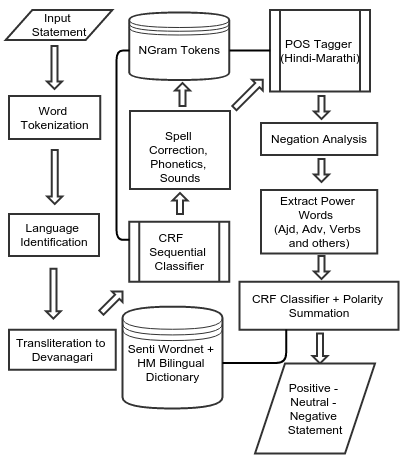
\includegraphics[width=90mm]{polarity-pickup.png}
    \caption{Flow diagram for the proposed approach}
\end{figure}


\subsection{Text Normalization}
Text normaliation step depends heavily on work of Srinivas
(\cite{sharma_text_2015}), which has following steps:
\begin{itemize*}
  \item \textbf{\textit{Language Identification}}; Tagging of the words as
      <word>/<tag>, where <tag> can be E or english, H for hindi and M or
      marathi,\\
  \item \textbf{\textit{Spelling Corrections}}; There are multipe ways to write
      Mujhe in hindi such as muze, muje, etc. To come to common and widely used
      spelling becomes very importnat\\
  \item \textbf{\textit{Ambiguous words}}; Words such as 'me' means same thing
      in english and marathi, where as in hindi it is sometimes used to say
      inside with another spelling being 'mein'. \\
  \item \textbf{\textit{Sounds}}; Words such as aww, oohh, ouch, ewww, etc.
      They do contain rich information when it comes to sentiments.\\
  \item \textbf{\textit{Phonetic words}}; Words such as pleej usually is
      misspelling of word please, spoken in some areas of the subcontinent. It
      gets written too in the similar manner.\\
  \item \textbf{\textit{Transliteration}}; Conversion of hindi/marathi words
      written in english to appropriate devnagari script.\\
\end{itemize*}

All then above enumerated steps have been covered by Srinivas
(\cite{sharma_text_2015}) and doesn't require us to go in the details of those,
however; we will look at some of those steps to get a proper grip on the
subject. At this point, this work will simply reuse those steps for hindi and try to
closely perform them for marathi as well. 

\subsubsection{Work-Token Normalization}
The process here is really simple to explain, but quite interesting to develop.
This is a required step as a sort of preprocessor, to enable the words to be
converted appropriately to their respective languages. Words like "awww",
"reaaaly", etc needs to be normalized and the techniques to do are covered by
Srinivas (\cite{sharma_text_2015} and \cite{shashank_sharma_sentiment_????}
) both. These methods are already tested with some accuracy in the above
mentioned papers themselves.  

\subsubsection{Language Identification Tagging}
The first step is to tag the language identifier for every word-token, using the techniques described in Kundu and Chandra et. al.
\cite{kundu_automatic_2012} and King and Abney \cite{king_labeling_2013}. The
output of this step will be more or less like in example given below:\\

\hspace{8em}"Yeh acchha din hai. Let's go now" \\
\hspace{8em}"Yeh|H acchha|H din|H hai|H. Let's|E go|E now|E". \\
To this effect, same approach can be accomplished for marathi text. Once we have tagged all the
word-tokens with their corresponding language identifier, we can move to next
step. However, there are going to be ambigious words "ho", "me", etc, which
shall use semi supervised learning for handing based on context. The plan is to
also test again HMM models to discover the accuracy difference.\\

\\
\hline
\textbf{ Algorithm: Language Identifier }
\hline
\begin{algorithmic}[1]
 \renewcommand{\algorithmicrequire}{\textbf{Input:}}
 \renewcommand{\algorithmicensure}{\textbf{Output:}}
 \REQUIRE word, sentence, languageDictionary
 \ENSURE  languageTag
 \\ \textbf{\textit{Initialization:}}
 \STATE le = TextCorpus.instance('English')
 \STATE ld = TextCorpus.instance('Devagiri')
 \STATE Xeh = Transliterator.instance('Hindi', 'English')
 \STATE Cd = TextCorpus.instance('DevangiriTransliterated')
 \STATE model = ConditionalRandomField.get(NGrammer.get(le), NGrammer.get(ld))
 \\ \textbf{\textit{Process:}}
 \IF {($word not in languageDictionary$)}
  \STATE word = MostSimilar(stem(word))
 \ENDIF
 \STATE langaugeTag = argMax(model, sentence, word)
 \RETURN $langageTag$
\end{algorithmic} 
\hline
\\

Language identification will be based on the approach of using hidden markov
models trained on the n-gram generated from corpus to be able to produce
probabilities for each work-token when considered with its neighbouring words
to identify the language to which the token belongs.\\

In all the related work \cite{shashank_sharma_sentiment_????}, there was a need
for transliteration mechanism in play on the fly. The reason for it being the
de facto method of choice is because it allows the usage of POS tagging to work
with the text, which would only \\
This database will be trained using hindi-english transliteration pairs
collected from Fire 2013 found at \cite{_linguistic_????} as well as result
of another previous work by Gupta et. al. \cite{gupta_mining_2012}. This
trained model will then be used to convert all the words in hindi wordnet to
ensure greater coverage of incoming input word tokens. In case of marathi, a
similar thing will be done and associated with hindi wordnet through
hindi-marathi bilingual dictionary.\\ 

\subsubsection{POS Tagging, Discourse analysis, Senti Word Net}
Before sentiment analysis can be performed, it is necessary to deal with few
important things. We are striving to extend and improve upon earlier work such
as Srinivas (\cite{sharma_text_2015}) and therefore following much in the same
footsteps. Both the step are explained further below.
Once we have the document in english or hindi, the next step is to run it
through POS tagger based on respective language. The approach will be straight
forward as detailed here \cite{vyas_pos_2014}. The POS Tagged prepositions
then shall be run through the negation discourse analysis to invert the POS
tagged adjectives and adverbs in case of negetive discourse as explained by Pandey
\cite{pandey_framework_2015} and Mittal et. al. \cite{mittal_sentiment_2013}.\\
\\
\hline
\textbf{ Algorithm: PolarityIdentification}
\hline
\begin{algorithmic}[1]
 \renewcommand{\algorithmicrequire}{\textbf{Input:}}
 \renewcommand{\algorithmicensure}{\textbf{Output:}}
 \REQUIRE sentence
 \ENSURE  dictionary
 \\ \textbf{\textit{Initialization:}}
 \STATE tagger = CombinedPOSTagger.instance()
 \STATE invPolarity = DiscourseAnalysis.instance()
 \STATE polarityLookup = SentimentPolarity.instance(['English', 'Hindi'])
 \\ \textbf{\textit{Process:}}
 sentenceTree = tagger.tagTree(sentence)
 sentencePTag = tagger.posTag(sentence)
 negation = False
 dictionary = []
 \FOR {$word$ in $sentencePTag$}
  \IF {(isEntity($word$))}
    \STATE continue
  \ENDIF
  \IF {(isNegetive($word$, $sentenceTree$))}
    \STATE negation = True
    \STATE continue
  \ENDIF
  \IF {($negetion$)}
    \STATE polarity = invPolarity(polarityLookup($word$))
  \ELSE
    \STATE polarity = polarityLookup($word$)
  \ENDIF
  dictionary.append(tuple($word$, $polarity$))
 \ENDFOR
 \RETURN $dictionary$
\end{algorithmic} 
\hline
\\

The output of POS Tagger shall be used to look up sentiword identifier for the
word groups using Sentiwordnet or HSWN, for English and Hindi, respectively.
HSWN has been improved by Pandey \cite{pandey_framework_2015} by making
additions to it and that will be used in this work. Here, there are three major
improvements we are considering. Since, it was established
\cite{shashank_sharma_sentiment_????} that the basis for sentiment analysis
being POS tagged adjectives and adverbs gives much better result that depending
direcly on lexicon or wordnet look up for each work, we would be going that
route. Secondly, addition of discourse analysis would further enhance on the
existing work \cite{shashank_sharma_sentiment_????}.
\\
\hline
\textbf{Algorithm: Polarity Classificiation}
\hline
\begin{algorithmic}[1]
 \renewcommand{\algorithmicrequire}{\textbf{Input:}}
 \renewcommand{\algorithmicensure}{\textbf{Output:}}
 \REQUIRE sentence
 \ENSURE  polarityProbability
 \\ \textbf{\textit{Initialization:}}
 \STATE naiveClassifier = NaiveBayesClassifier .trainedInstance()
 \STATE linearClassifer = LinearSummation .instance()
 \\ \textbf{\textit{Process:}}
 \STATE wordDictionary = PolarityIndentification (sentence)
 \STATE polarityProbability = [ naiveClassifier(wordDict), linearClassifer(wordDict) ]
 \RETURN $polarityProbability$
\end{algorithmic} 
\hline
\\

\subsubsection{Sentiment classification using classifier}
Once we get sentiword identifier for each token - word, next step is to put it
through the classifier which will give the polartiy of the statement provided.
This polarity checking decision can be as simple as simple summation of all
word-token sentiment polarities or further analysis can be performed to figure
out what really is the polarity of word-token and its membership with negetive,
postive or neutral . This step being the vital one can be accomplished using
most trust classifier like SVM, Random Forests, however; impetus shall be given
on naive bayes classifier for brevity's sake. \\

\\
\textbf{Example Flow: }
\hline
\begin{algorithmic}[1]
 \renewcommand{\algorithmicrequire}{\textbf{Input:}}
 \REQUIRE 'Kitni der se ticket cancel nahi ho rahi hai'\\
 \\ \textbf{\textit{Language Identification:} }
 \\ kitni|H der|H se|H ticket|E cancel|E nahi|H ho|H rahi|H hai|H
 \\ \textbf{\textit{Transliteration: }} 
   \foreignlanguage{sanskrit}{
कितनी देर से
}
ticket cancel
\foreignlanguage{sanskrit}{
नहीं हो रही है  
}\\
\\ \textbf{\textit{POS Hindi:}}\\
\foreignlanguage{sanskrit}{कितनी}|adj - QF\\
\foreignlanguage{sanskrit}{देर}|adv - NN\\
\foreignlanguage{sanskrit}{से}|v - PSP\\
ticket|unk - JJ\\
cancel|unk - NN\\
\foreignlanguage{sanskrit}{नहीं}|adv - NEG\\
\foreignlanguage{sanskrit}{हो}|v - VM\\
\foreignlanguage{sanskrit}{रही}|v - VAUX\\
\foreignlanguage{sanskrit}{है}|v - VAUX\\

\\ \textbf{\textit{Negation discourse analysis:}} \\
\foreignlanguage{sanskrit}{नहीं} and \foreignlanguage{sanskrit}{हो} are closely
associated with one another. Negation discourse analysis works on the subtree
level, which in this case is post the word \foreignlanguage{sanskrit}{हो} a. \\
So all the words following 'nahi' will be part of it's subtree. Hence, all the
polarity from that point onwards will be reverse.

\\\textbf{\textit{Poliarity extraction example:}} \\
polarity = \foreignlanguage{sanskrit}{कितनी}|adj=INC
\foreignlanguage{sanskrit}{देर}|adv=NEG \foreignlanguage{sanskrit}{से}|v=NEU
ticket|NN=Neu cancel|=NEG \foreignlanguage{sanskrit}{नहीं}|adv=NEG
\foreignlanguage{sanskrit}{हो}|v=NEU  \foreignlanguage{sanskrit}{रही}|v=NEU
\foreignlanguage{sanskrit}{है}|v=NEU\\ 
polarity = (INC * NEG) + NEU + NEG + [NEG:REVERSE + NEU + NEU + NEU]\\
polarity = (2 * -1) + 0 + -1 + (-1 * (0 + 0 + 0))\\
polarity = -2 + 0 -1 + (-1 * 0)\\
polarity = -2 -1 + 0\\
polarity = -3\\

\end{algorithmic} 
\hline
\\
Quite clearly, we have input as POS tagged statements with greater emphasis on
adjectives and adverbs that are inverted in case of negation present in the
preposition. Once we have this tagged information, we would like to test on
both the process of simple polarity count summation of the given input and
traning the classifier, in order to come up with the best possible result in
terms of accuracy.\\



% An example of a floating figure using the graphicx package.
% Note that \label must occur AFTER (or within) \caption.
% For figures, \caption should occur after the \includegraphics.
% Note that IEEEtran v1.7 and later has special internal code that
% is designed to preserve the operation of \label within \caption
% even when the captionsoff option is in effect. However, because
% of issues like this, it may be the safest practice to put all your
% \label just after \caption rather than within \caption{}.
%
% Reminder: the "draftcls" or "draftclsnofoot", not "draft", class
% option should be used if it is desired that the figures are to be
% displayed while in draft mode.
%
%\begin{figure}[!t]
%\centering
%\includegraphics[width=2.5in]{myfigure}
% where an .eps filename suffix will be assumed under latex, 
% and a .pdf suffix will be assumed for pdflatex; or what has been declared
% via \DeclareGraphicsExtensions.
%\caption{Simulation results for the network.}
%\label{fig_sim}
%\end{figure}

% Note that the IEEE typically puts floats only at the top, even when this
% results in a large percentage of a column being occupied by floats.


% An example of a double column floating figure using two subfigures.
% (The subfig.sty package must be loaded for this to work.)
% The subfigure \label commands are set within each subfloat command,
% and the \label for the overall figure must come after \caption.
% \hfil is used as a separator to get equal spacing.
% Watch out that the combined width of all the subfigures on a 
% line do not exceed the text width or a line break will occur.
%
%\begin{figure*}[!t]
%\centering
%\subfloat[Case I]{\includegraphics[width=2.5in]{box}%
%\label{fig_first_case}}
%\hfil
%\subfloat[Case II]{\includegraphics[width=2.5in]{box}%
%\label{fig_second_case}}
%\caption{Simulation results for the network.}
%\label{fig_sim}
%\end{figure*}
%
% Note that often IEEE papers with subfigures do not employ subfigure
% captions (using the optional argument to \subfloat[]), but instead will
% reference/describe all of them (a), (b), etc., within the main caption.
% Be aware that for subfig.sty to generate the (a), (b), etc., subfigure
% labels, the optional argument to \subfloat must be present. If a
% subcaption is not desired, just leave its contents blank,
% e.g., \subfloat[].


% An example of a floating table. Note that, for IEEE style tables, the
% \caption command should come BEFORE the table and, given that table
% captions serve much like titles, are usually capitalized except for words
% such as a, an, and, as, at, but, by, for, in, nor, of, on, or, the, to
% and up, which are usually not capitalized unless they are the first or
% last word of the caption. Table text will default to \footnotesize as
% the IEEE normally uses this smaller font for tables.
% The \label must come after \caption as always.
%
%\begin{table}[!t]
%% increase table row spacing, adjust to taste
%\renewcommand{\arraystretch}{1.3}
% if using array.sty, it might be a good idea to tweak the value of
% \extrarowheight as needed to properly center the text within the cells
%\caption{An Example of a Table}
%\label{table_example}
%\centering
%% Some packages, such as MDW tools, offer better commands for making tables
%% than the plain LaTeX2e tabular which is used here.
%\begin{tabular}{|c||c|}
%\hline
%One & Two\\
%\hline
%Three & Four\\
%\hline
%\end{tabular}
%\end{table}


% Note that the IEEE does not put floats in the very first column
% - or typically anywhere on the first page for that matter. Also,
% in-text middle ("here") positioning is typically not used, but it
% is allowed and encouraged for Computer Society conferences (but
% not Computer Society journals). Most IEEE journals/conferences use
% top floats exclusively. 
% Note that, LaTeX2e, unlike IEEE journals/conferences, places
% footnotes above bottom floats. This can be corrected via the
% \fnbelowfloat command of the stfloats package.




\section{Conclusion}
The most important aspect of this work i.e. the results are what is coming
next. We will show that the approach proposed in this work performs better than
all the work presented here in literature, when considered independently. It is
the synergy, which the approach presented there, promises. The implementation
will happen for all ways that differ from the approach too, so that comparisons
can be made and conclusions drawn without the strawman arguments. 


There is a lot of work to be performed before any concrete conclusion can be
expressed, however; There is a great possibility that the approach suggested in
the given work will result in improvement in the field of sentiment analysis,
that can again be extended for greater language coverage in as well as out of
indian languages. These strides towards such improvements will result in
machine's being able to understand human sentiments better, which is one of the
greatest challenge being faced by the research in general AI. Ours is but a
small step towards that goal. It will not be too far fetched to believe that
the improvements will range from 5 to 10 percent improvement where we will see
the accuracy reach 95 percent. \\




% conference papers do not normally have an appendix


% use section* for acknowledgment
%\section*{Acknowledgment}
%The authors would like to thank...





% trigger a \newpage just before the given reference
% number - used to balance the columns on the last page
% adjust value as needed - may need to be readjusted if
% the document is modified later
%\IEEEtriggeratref{8}
% The "triggered" command can be changed if desired:
%\IEEEtriggercmd{\enlargethispage{-5in}}

% references section

% can use a bibliography generated by BibTeX as a .bbl file
% BibTeX documentation can be easily obtained at:
% http://mirror.ctan.org/biblio/bibtex/contrib/doc/
% The IEEEtran BibTeX style support page is at:
% http://www.michaelshell.org/tex/ieeetran/bibtex/
%\bibliographystyle{IEEEtran}
% argument is your BibTeX string definitions and bibliography database(s)
%\bibliography{IEEEabrv,../bib/paper}
%
% <OR> manually copy in the resultant .bbl file
% set second argument of \begin to the number of references
% (used to reserve space for the reference number labels box)
%\begin{thebibliography}{1}
%\bibitem{IEEEhowto:kopka}
%H.~Kopka and P.~W. Daly, \emph{A Guide to \LaTeX}, 3rd~ed.\hskip 1em plus
  %0.5em minus 0.4em\relax Harlow, England: Addison-Wesley, 1999.

%\end{thebibliography}


%\bibliographystyle{IEEEtran}
%\bibliography{IEEEabrv,report}
\printbibliography


% that's all folks
\end{document}


